\documentclass[11pt]{article}
\usepackage[margin=1in]{geometry}
\usepackage{graphicx}
\usepackage{enumitem}
\usepackage{booktabs}
\usepackage{hyperref}
\usepackage{xcolor}
\usepackage{caption}
\usepackage{tikz}
\usetikzlibrary{arrows.meta,positioning}

\hypersetup{
  colorlinks=true,
  linkcolor=blue,
  urlcolor=magenta
}

\title{CS 3642 Programming Assignment 1\\
\large Boids with Predator (Shark) in Go + WebAssembly}
\date{} 

\begin{document}
\maketitle

\noindent
\textbf{Course:} CS 3642 --- Artificial Intelligence\\
\textbf{Student:} James Widner\\
\textbf{ID:} 001121770\\
\textbf{Date: }\date{\today}

\section*{Section 1: Agent Design}

\subsection*{Overview: Why This Is Model-Based}
My implementation has two kinds of agents:

\begin{itemize}[leftmargin=1.25em]
  \item \textbf{Boids (fish):} each fish stores position, velocity, tail history, and alive/dead state. They move according to the three classic boids rules: separation, alignment, and cohesion, plus additional models for wall avoidance, a gentle pull to the center, and predator avoidance.
  \item \textbf{Shark (predator):} stores its own position, velocity, patrol phase, smoothed patrol center, and an eating cooldown timer. In patrol mode, it follows an elliptical orbit around the flock using PD control. In evil mode, it performs lead pursuit and can eat boids inside a radius, incrementing a score.
\end{itemize}

Because both agents use internal state (e.g., flock centroid, wall lookahead, patrol phase, cooldown timer) to choose actions, this is a \textbf{model-based agent system}.

\subsection*{Finite-State Diagram (Predator)}
\begin{center}
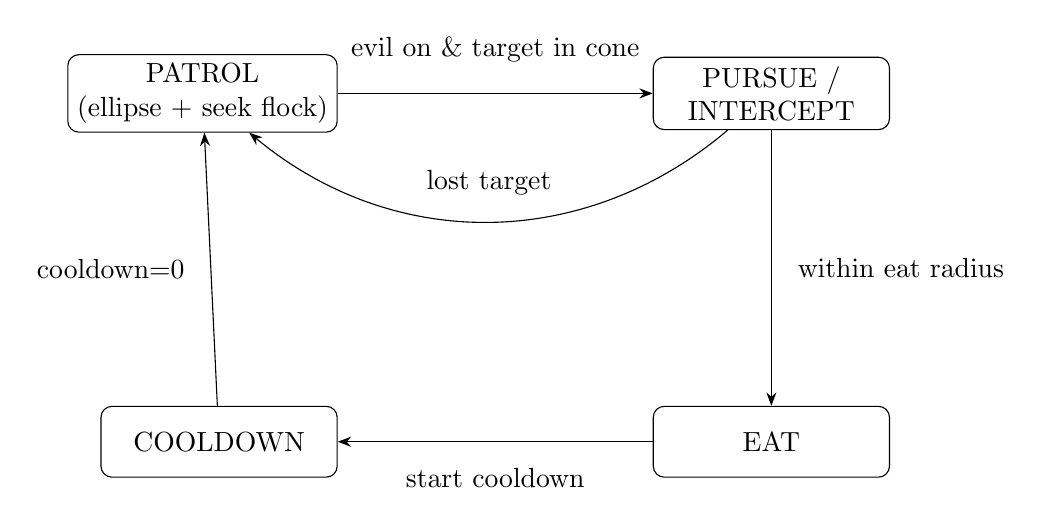
\begin{tikzpicture}[
  node distance=35mm and 40mm, 
  >=Stealth,
  state/.style={rectangle,rounded corners,draw,align=center,minimum width=30mm,minimum height=9mm}
]
\node[state] (patrol) {PATROL\\(ellipse + seek flock)};
\node[state, right=of patrol] (pursue) {PURSUE /\\INTERCEPT};
\node[state, below=of pursue] (eat) {EAT};
\node[state, left=of eat] (cool) {COOLDOWN};

% arrows
\draw[->] (patrol) -- node[above=8pt, align=center]{evil on \& target in cone} (pursue);
\draw[->] (pursue) -- node[right=6pt, align=center]{within eat radius} (eat);
\draw[->] (eat) -- node[below=6pt]{start cooldown} (cool);
\draw[->] (cool) -- node[left=6pt]{cooldown=0} (patrol);
\draw[->, bend left=40] (pursue) to node[above=6pt]{lost target} (patrol);
\end{tikzpicture}
\end{center}

\subsection*{Internal Models (Summary)}
The three core rules come from Reynolds' boids model (1987), popularized in tutorials such as Sebastian Lague's \emph{Boids} project. A related fish-schooling formulation appears in Inada (2001).
I did not derive these equations; I implemented and tuned them for this simulation. In words:

\begin{itemize}[leftmargin=1.25em]
  \item \textbf{Separation:} steer away from nearby boids to avoid collisions.
  \item \textbf{Alignment:} steer to match the average velocity of neighbors.
  \item \textbf{Cohesion:} steer toward the average position of neighbors.
\end{itemize}

Additional models I added:
\begin{itemize}[leftmargin=1.25em]
  \item \textbf{Wall avoidance:} predictive steering away from world boundaries using a blended wall normal.
  \item \textbf{Home field:} gentle pull back toward the center of the canvas.
  \item \textbf{Predator avoidance:} flee when the shark enters a threat radius.
  \item \textbf{Predator behavior:} elliptical PD patrol, flock-seeking bias, evil-mode interception, eating cooldown, and score tracking.
\end{itemize}

\subsection*{PEAS for Predator}
\begin{tabular}{@{}p{0.18\linewidth}p{0.78\linewidth}@{}}
\toprule
\textbf{Performance} & 
Smooth patrol paths, staying near the flock, successful captures in evil mode, natural-looking motion (turn/force bounded), and no wall penetration. \\
\midrule
\textbf{Environment} & 
2D continuous bounded world; 48 boids using Reynolds-style rules (separation, alignment, cohesion); stochastic jitter; predator present. \\
\midrule
\textbf{Actuators} & 
Velocity steering (bounded by max turn and max force); mode toggle (patrol vs evil); cooldown timer for eating. \\
\midrule
\textbf{Sensors} & 
Own position/velocity; flock centroid; nearby boid positions/velocities (with FOV and radius limits); wall proximity (via predictive normal); slider/checkbox inputs from the GUI. \\
\bottomrule
\end{tabular}

\section*{Section 2: Tasks}

\paragraph{Task 1 — Cohesive flocking in a bounded 2D world.}
Boids maintain a stable school using separation, alignment, and cohesion plus predictive wall avoidance and a center pull.  
\emph{Measure:} average speed stability, cluster compactness, low collisions.

\paragraph{Task 2 — Predator patrol (benign).}
The shark follows an ellipse around the flock centroid using PD control with a small group-seeking bias.  
\emph{Measure:} smoothness of path, proximity to flock, natural motion.

\paragraph{Task 3 — Interception and eating (evil mode).}
In evil mode, the shark selects a forward target, performs lead pursuit with a sweep bias, and eats if within radius, with a cooldown.  
\emph{Measure:} number of captures (score), time-to-capture, believability of pursuit.

\paragraph{Task 4 — Human-in-the-loop control.}
Sliders adjust rule weights, separation radius, shark speed, patrol scale, bias, group-seek, and tail length. Checkbox toggles evil mode.  
\emph{Measure:} UI responsiveness, smooth live updates at $\sim$60 FPS.

\section*{Section 3: Codes and Outputs}

\subsection*{Implementation Notes}
\begin{itemize}[leftmargin=1.25em]
  \item Implemented in Go, compiled to WebAssembly.
  \item Core types: \texttt{Vec2}, \texttt{Boid}, \texttt{Shark}.
  \item Main loop: read sliders $\rightarrow$ update flock centroid $\rightarrow$ update shark (patrol/pursuit) $\rightarrow$ boid updates $\rightarrow$ render.
  \item Rendering: sprites for boids, tails, shark. Score updated live via JS.
\end{itemize}

\subsection*{Repository and Demo}
Source code: \url{https://github.com/pi128/CS3642} \\
Live WASM demo: \url{https://pi128.github.io/CS3642/} \\
Original plan: port to my \emph{FreeWiLi} device; code is organized to enable that deployment. Unable to flash device for WASM files :(


\begin{figure}[h]
  \centering
  
 
  
\includegraphics[width=0.8\linewidth]{fish.png}
  \caption{Simulation running with flock and shark.}
\end{figure}

\newpage

\section*{Discussion, Limitations, and Future Work}
The classic boids rules (separation, alignment, cohesion) were adapted from prior work (Reynolds 1987; Lague's Boids repo; Inada 2001). My additions include predictive wall avoidance, a home field, and the predator with two modes.

\textbf{Limitations:} In evil mode, the shark can still move somewhat erratically due to rapid target switching and aggressive lead pursuit. Boids are all identical and lack behavioral states (panic vs cruise).

\textbf{Future work:} Add hysteresis or dwell time for target switching, smooth the shark's desired velocity to reduce jitter, explore multi-predator dynamics, implement spatial partitioning (e.g., grids) for scalability, and complete the FreeWiLi port.

\section*{References}
\begin{itemize}[leftmargin=1.25em]
  \item C.\,W. Reynolds, ``Flocks, Herds, and Schools: A Distributed Behavioral Model,'' \emph{Computer Graphics} 21(4), 1987.
  \item Sebastian Lague, \emph{Boids} (GitHub repo). URL: \url{https://github.com/SebLague/Boids}
  \item Y. Inada, ``Steering Mechanism of Fish Schools,'' \emph{Complexity International}, vol. 8, 2001. (PDF available online)
\end{itemize}
\section*{Academic Honesty Statement}
I affirm that this report and the associated code were prepared by me,
James Widner (ID: 001121770), for CS 3642. 

I clearly distinguish between:
\begin{itemize}[leftmargin=1.25em]
  \item Ideas and rules adapted from prior work: Reynolds' boids model (1987),
  Sebastian Lague's Boids repository, and Inada's 2001 fish-schooling paper.
  \item My own contributions: implementation in Go/WASM, predictive wall
  avoidance, home-field steering, stochastic jitter, and the predator (shark)
  with elliptical PD patrol, flock-seeking bias, evil-mode interception,
  cooldown eating, and UI slider integration.
\end{itemize}

I hope this work complies with the academic integrity policies of CS 3642. I
started this project in late August then this assignment came up and I thought it would be a good challenge.

\end{document}